Hierarhija sistema datoteka ili Filesystem Hierarchy Standard (FHS) definiše strukturu foldera u Linux sistemima. U FSH-u, svi fajlovi i folderi se nalaze u \texttt{root} foleru (označen kao \texttt{/}), rasporedjeni po specifičnim subfolderima na osnovu njihove funkcije.
\begin{itemize}
\item \texttt{/bin} - sadrži neophodne programe na sistemu, kao \texttt{cat}, \texttt{ls}, \texttt{cp}.

\item \texttt{/boot} - fajlovi za bootloader

\item \texttt{/dev} - fajlovi neophodni za koriscenje uredjaja.

\item \texttt{/etc} - fajlovi za konfiguraciju programa i procesa.

\item \texttt{/home} - svi fajlovi i folderi korsnika

\item \texttt{/lib} - "biblioteke" neophodne za pokretanje programa iz \texttt{/bin}.

\item \texttt{/media} - namenjen za pristup sadržaju priključenih uredjaja, kao fleš drajvova, CD-ROM-ova, itd.

\item \texttt{/mnt} - namenjano za pristup privremenim uredjaja

\item \texttt{/proc} - sadrži inforamacije o sistemskim procesima i kernel-u u obliku fajlova.

\item \texttt{/usr} - sadrži sve instalirane programe koji se ne nalaze u \texttt{/bin}.

\item \texttt{/var} - "promenljivi" fajlovi - fajlovi koji beleže razne promene i podatke tokom rada.

\item \texttt{/tmp} - privremeni fajlovi i folderi koji se brišu pri gašenju sistema.

\begin{figure}[H]
	\centering
	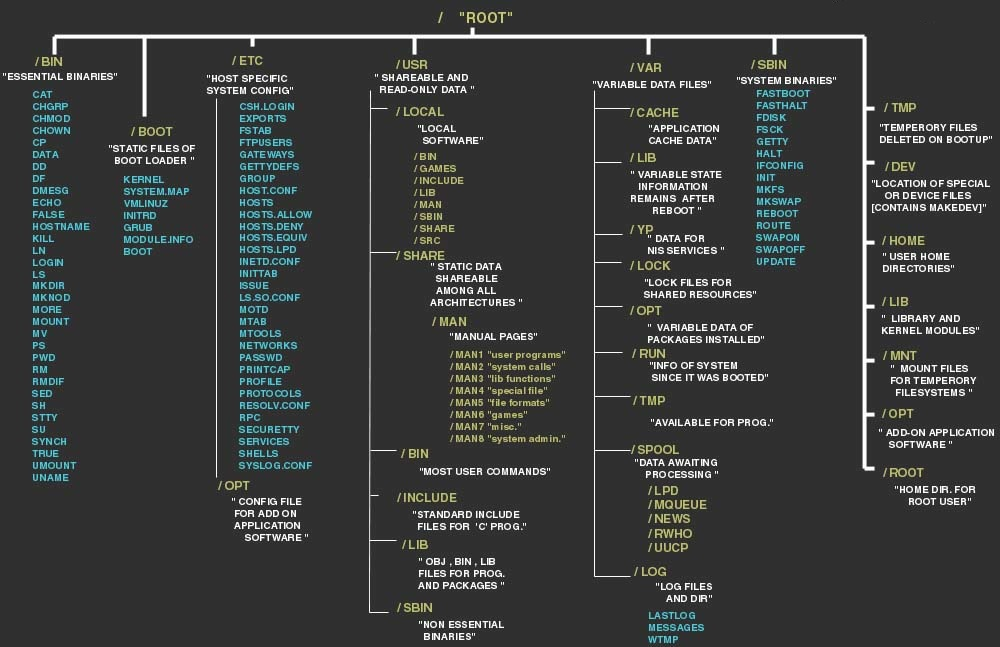
\includegraphics[width=\textwidth]{folders}
	\caption{Vizuelno predstavljena hierarhija sistema datoteka}
\end{figure}

\end{itemize}